\documentclass[border=10pt]{standalone}
\usepackage[utf8]{inputenc}
\usepackage{tikz}
\usetikzlibrary{positioning, arrows.meta, calc, fit, backgrounds, shapes.geometric, decorations.pathreplacing, patterns}
\usepackage{amsmath, amssymb}
\usepackage{xcolor}

% Colors
\definecolor{bg}{HTML}{F8F9FA}
\definecolor{inputcol}{HTML}{4488FF}
\definecolor{convcol}{HTML}{FF6B35}
\definecolor{bncol}{HTML}{FFB347}
\definecolor{poolcol}{HTML}{87CEEB}
\definecolor{gapcol}{HTML}{9B59B6}
\definecolor{dropcol}{HTML}{95A5A6}
\definecolor{fccol}{HTML}{E74C3C}
\definecolor{grucol}{HTML}{2ECC71}
\definecolor{featcol}{HTML}{F39C12}
\definecolor{svmcol}{HTML}{8E44AD}
\definecolor{rfcol}{HTML}{27AE60}
\definecolor{scalecol}{HTML}{3498DB}
\definecolor{arrowcol}{HTML}{2C3E50}
\definecolor{textgray}{HTML}{555555}
\definecolor{dimcol}{HTML}{888888}

\begin{document}

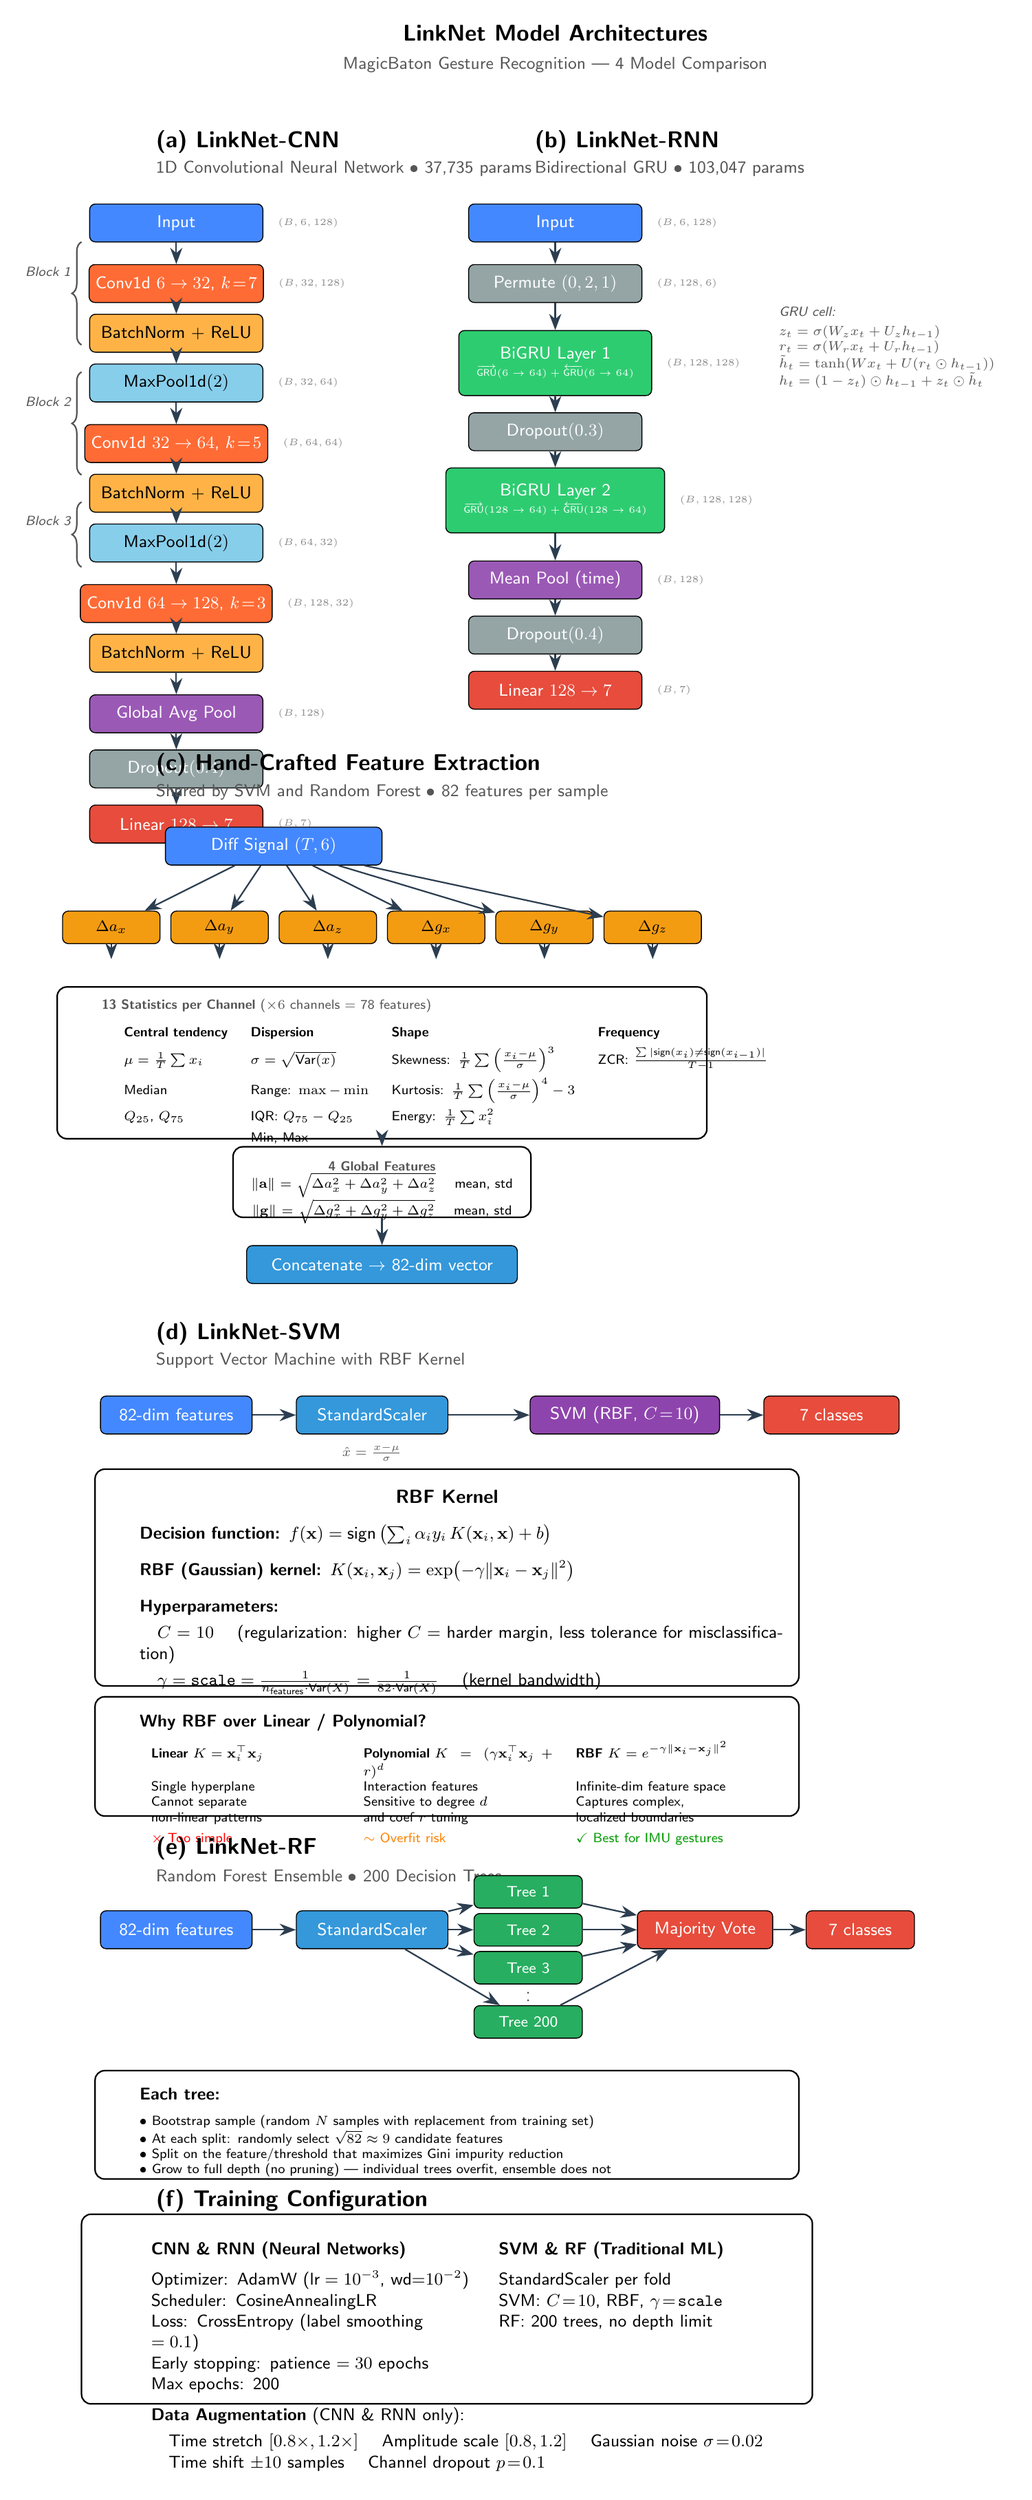
\begin{tikzpicture}[
    node distance=0.5cm,
    >={Stealth[length=3mm]},
    block/.style={draw, rounded corners=3pt, minimum width=3.2cm, minimum height=0.7cm,
                  font=\small\sffamily, text=white, line width=0.5pt},
    dim/.style={font=\tiny\sffamily\color{dimcol}, anchor=west},
    label/.style={font=\scriptsize\sffamily\color{textgray}},
    title/.style={font=\large\sffamily\bfseries},
    subtitle/.style={font=\small\sffamily\color{textgray}},
    arrow/.style={->, arrowcol, line width=0.8pt},
    dasharrow/.style={->, arrowcol, line width=0.6pt, dashed},
]

% ============================================================
% TITLE
% ============================================================
\node[title] (maintitle) at (7, 1) {LinkNet Model Architectures};
\node[subtitle, below=0.05cm of maintitle] {MagicBaton Gesture Recognition --- 4 Model Comparison};

% ============================================================
% CNN
% ============================================================
\begin{scope}[shift={(0, -1.5)}]
    \node[title, anchor=west] at (-0.5, 0.5) {(a) LinkNet-CNN};
    \node[subtitle, anchor=west] at (-0.5, 0) {1D Convolutional Neural Network \textbullet\ 37,735 params};

    % Input
    \node[block, fill=inputcol] (cin) at (0, -1) {Input};
    \node[dim, right=0.15cm of cin] {$(B, 6, 128)$};

    % Block 1
    \node[block, fill=convcol, below=0.4cm of cin] (c1) {Conv1d $6 \to 32$, $k\!=\!7$};
    \node[dim, right=0.15cm of c1] {$(B, 32, 128)$};

    \node[block, fill=bncol, text=black, below=0.2cm of c1] (bn1) {BatchNorm + ReLU};

    \node[block, fill=poolcol, text=black, below=0.2cm of bn1] (p1) {MaxPool1d$(2)$};
    \node[dim, right=0.15cm of p1] {$(B, 32, 64)$};

    % Block 2
    \node[block, fill=convcol, below=0.4cm of p1] (c2) {Conv1d $32 \to 64$, $k\!=\!5$};
    \node[dim, right=0.15cm of c2] {$(B, 64, 64)$};

    \node[block, fill=bncol, text=black, below=0.2cm of c2] (bn2) {BatchNorm + ReLU};

    \node[block, fill=poolcol, text=black, below=0.2cm of bn2] (p2) {MaxPool1d$(2)$};
    \node[dim, right=0.15cm of p2] {$(B, 64, 32)$};

    % Block 3
    \node[block, fill=convcol, below=0.4cm of p2] (c3) {Conv1d $64 \to 128$, $k\!=\!3$};
    \node[dim, right=0.15cm of c3] {$(B, 128, 32)$};

    \node[block, fill=bncol, text=black, below=0.2cm of c3] (bn3) {BatchNorm + ReLU};

    % GAP
    \node[block, fill=gapcol, below=0.4cm of bn3] (gap) {Global Avg Pool};
    \node[dim, right=0.15cm of gap] {$(B, 128)$};

    % Dropout + FC
    \node[block, fill=dropcol, below=0.3cm of gap] (drop) {Dropout$(0.4)$};

    \node[block, fill=fccol, below=0.3cm of drop] (fc) {Linear $128 \to 7$};
    \node[dim, right=0.15cm of fc] {$(B, 7)$};

    % Arrows
    \foreach \a/\b in {cin/c1, c1/bn1, bn1/p1, p1/c2, c2/bn2, bn2/p2, p2/c3, c3/bn3, bn3/gap, gap/drop, drop/fc}{
        \draw[arrow] (\a) -- (\b);
    }

    % Block labels
    \node[label, anchor=east] at (-1.8, -1.9) {\textit{Block 1}};
    \node[label, anchor=east] at (-1.8, -4.3) {\textit{Block 2}};
    \node[label, anchor=east] at (-1.8, -6.5) {\textit{Block 3}};

    % Braces
    \draw[decorate, decoration={brace, amplitude=5pt, mirror}, thick, textgray]
        (-1.75, -1.35) -- (-1.75, -3.25) ;
    \draw[decorate, decoration={brace, amplitude=5pt, mirror}, thick, textgray]
        (-1.75, -3.75) -- (-1.75, -5.65) ;
    \draw[decorate, decoration={brace, amplitude=5pt, mirror}, thick, textgray]
        (-1.75, -6.15) -- (-1.75, -7.35) ;
\end{scope}

% ============================================================
% RNN
% ============================================================
\begin{scope}[shift={(7, -1.5)}]
    \node[title, anchor=west] at (-0.5, 0.5) {(b) LinkNet-RNN};
    \node[subtitle, anchor=west] at (-0.5, 0) {Bidirectional GRU \textbullet\ 103,047 params};

    % Input
    \node[block, fill=inputcol] (rin) at (0, -1) {Input};
    \node[dim, right=0.15cm of rin] {$(B, 6, 128)$};

    % Permute
    \node[block, fill=dropcol, below=0.4cm of rin] (perm) {Permute $(0,2,1)$};
    \node[dim, right=0.15cm of perm] {$(B, 128, 6)$};

    % GRU Layer 1
    \node[block, fill=grucol, below=0.5cm of perm, minimum height=1.2cm] (gru1) {%
        \begin{tabular}{c}
        BiGRU Layer 1 \\[-2pt]
        {\tiny $\overrightarrow{\text{GRU}}(6 \to 64) + \overleftarrow{\text{GRU}}(6 \to 64)$}
        \end{tabular}};
    \node[dim, right=0.15cm of gru1] {$(B, 128, 128)$};

    % Dropout between layers
    \node[block, fill=dropcol, below=0.3cm of gru1] (gdrop1) {Dropout$(0.3)$};

    % GRU Layer 2
    \node[block, fill=grucol, below=0.3cm of gdrop1, minimum height=1.2cm] (gru2) {%
        \begin{tabular}{c}
        BiGRU Layer 2 \\[-2pt]
        {\tiny $\overrightarrow{\text{GRU}}(128 \to 64) + \overleftarrow{\text{GRU}}(128 \to 64)$}
        \end{tabular}};
    \node[dim, right=0.15cm of gru2] {$(B, 128, 128)$};

    % Mean pool
    \node[block, fill=gapcol, below=0.5cm of gru2] (rmean) {Mean Pool (time)};
    \node[dim, right=0.15cm of rmean] {$(B, 128)$};

    % Dropout + FC
    \node[block, fill=dropcol, below=0.3cm of rmean] (rdrop) {Dropout$(0.4)$};

    \node[block, fill=fccol, below=0.3cm of rdrop] (rfc) {Linear $128 \to 7$};
    \node[dim, right=0.15cm of rfc] {$(B, 7)$};

    % Arrows
    \foreach \a/\b in {rin/perm, perm/gru1, gru1/gdrop1, gdrop1/gru2, gru2/rmean, rmean/rdrop, rdrop/rfc}{
        \draw[arrow] (\a) -- (\b);
    }

    % GRU internal diagram
    \node[label, anchor=west] at (3.8, -3.3) {%
        \begin{tabular}{l}
        \textit{GRU cell:} \\[2pt]
        $z_t = \sigma(W_z x_t + U_z h_{t-1})$ \\
        $r_t = \sigma(W_r x_t + U_r h_{t-1})$ \\
        $\tilde{h}_t = \tanh(W x_t + U(r_t \odot h_{t-1}))$ \\
        $h_t = (1-z_t) \odot h_{t-1} + z_t \odot \tilde{h}_t$
        \end{tabular}};
\end{scope}

% ============================================================
% Feature Extraction (for SVM / RF)
% ============================================================
\begin{scope}[shift={(0, -13)}]
    \node[title, anchor=west] at (-0.5, 0.5) {(c) Hand-Crafted Feature Extraction};
    \node[subtitle, anchor=west] at (-0.5, 0) {Shared by SVM and Random Forest \textbullet\ 82 features per sample};

    % Input
    \node[block, fill=inputcol, minimum width=4cm] (fin) at (1.8, -1) {Diff Signal $(T, 6)$};

    % Split into channels
    \node[block, fill=featcol, text=black, minimum width=1.8cm, minimum height=0.6cm]
        (ch0) at (-1.2, -2.5) {\footnotesize $\Delta a_x$};
    \node[block, fill=featcol, text=black, minimum width=1.8cm, minimum height=0.6cm]
        (ch1) at (0.8, -2.5) {\footnotesize $\Delta a_y$};
    \node[block, fill=featcol, text=black, minimum width=1.8cm, minimum height=0.6cm]
        (ch2) at (2.8, -2.5) {\footnotesize $\Delta a_z$};
    \node[block, fill=featcol, text=black, minimum width=1.8cm, minimum height=0.6cm]
        (ch3) at (4.8, -2.5) {\footnotesize $\Delta g_x$};
    \node[block, fill=featcol, text=black, minimum width=1.8cm, minimum height=0.6cm]
        (ch4) at (6.8, -2.5) {\footnotesize $\Delta g_y$};
    \node[block, fill=featcol, text=black, minimum width=1.8cm, minimum height=0.6cm]
        (ch5) at (8.8, -2.5) {\footnotesize $\Delta g_z$};

    \foreach \c in {ch0,ch1,ch2,ch3,ch4,ch5}{
        \draw[arrow] (fin) -- (\c);
    }

    % Stats box
    \node[draw, rounded corners=5pt, minimum width=12cm, minimum height=2.8cm,
          fill=white, line width=0.8pt] (statsbox) at (3.8, -5) {};
    \node[label, anchor=north west] at (-1.5, -3.7) {\textbf{13 Statistics per Channel} ($\times 6$ channels = 78 features)};

    \node[font=\scriptsize\sffamily, anchor=north west, text width=11cm] at (-1.3, -4.2) {%
        \begin{tabular}{llll}
        \textbf{Central tendency} & \textbf{Dispersion} & \textbf{Shape} & \textbf{Frequency} \\[3pt]
        $\mu = \frac{1}{T}\sum x_i$ & $\sigma = \sqrt{\text{Var}(x)}$ & Skewness: $\frac{1}{T}\sum\left(\frac{x_i-\mu}{\sigma}\right)^3$ & ZCR: $\frac{\sum|\text{sign}(x_i) \neq \text{sign}(x_{i-1})|}{T-1}$ \\[5pt]
        Median & Range: $\max - \min$ & Kurtosis: $\frac{1}{T}\sum\left(\frac{x_i-\mu}{\sigma}\right)^4 - 3$ & \\[5pt]
        $Q_{25}$, $Q_{75}$ & IQR: $Q_{75} - Q_{25}$ & Energy: $\frac{1}{T}\sum x_i^2$ & \\[3pt]
        & Min, Max & & \\
        \end{tabular}
    };

    % Arrows from channels to stats
    \foreach \c in {ch0,ch1,ch2,ch3,ch4,ch5}{
        \draw[arrow] (\c) -- ([yshift=0.5cm]\c |- statsbox.north);
    }

    % Global features
    \node[draw, rounded corners=5pt, minimum width=5.5cm, minimum height=1.3cm,
          fill=white, line width=0.8pt] (globalbox) at (3.8, -7.2) {};
    \node[label, anchor=north] at (3.8, -6.7) {\textbf{4 Global Features}};
    \node[font=\scriptsize\sffamily, text width=5cm, align=center] at (3.8, -7.5) {%
        $\|\mathbf{a}\| = \sqrt{\Delta a_x^2 + \Delta a_y^2 + \Delta a_z^2}$ \quad mean, std \\
        $\|\mathbf{g}\| = \sqrt{\Delta g_x^2 + \Delta g_y^2 + \Delta g_z^2}$ \quad mean, std
    };

    \draw[arrow] (statsbox) -- (globalbox);

    % Concatenate
    \node[block, fill=scalecol, minimum width=5cm, below=0.5cm of globalbox] (concat) {Concatenate $\to$ 82-dim vector};
    \draw[arrow] (globalbox) -- (concat);
\end{scope}

% ============================================================
% SVM
% ============================================================
\begin{scope}[shift={(0, -23.5)}]
    \node[title, anchor=west] at (-0.5, 0.5) {(d) LinkNet-SVM};
    \node[subtitle, anchor=west] at (-0.5, 0) {Support Vector Machine with RBF Kernel};

    % Pipeline
    \node[block, fill=inputcol, minimum width=2.8cm] (sin) at (0, -1) {82-dim features};

    \node[block, fill=scalecol, minimum width=2.8cm, right=0.8cm of sin] (sscale) {StandardScaler};
    \node[label, below=0.05cm of sscale] {$\hat{x} = \frac{x - \mu}{\sigma}$};

    \node[block, fill=svmcol, minimum width=3.5cm, right=1.5cm of sscale] (ssvm) {SVM (RBF, $C\!=\!10$)};

    \node[block, fill=fccol, minimum width=2.5cm, right=0.8cm of ssvm] (sout) {7 classes};

    \draw[arrow] (sin) -- (sscale);
    \draw[arrow] (sscale) -- (ssvm);
    \draw[arrow] (ssvm) -- (sout);

    % RBF Kernel explanation
    \node[draw, rounded corners=5pt, minimum width=13cm, minimum height=4cm,
          fill=white, line width=0.8pt] (rbfbox) at (5, -4) {};
    \node[title, font=\normalsize\sffamily\bfseries] at (5, -2.5) {RBF Kernel};

    \node[font=\small\sffamily, text width=12cm, anchor=north west] at (-0.8, -2.9) {%
        \textbf{Decision function:} $f(\mathbf{x}) = \text{sign}\left(\sum_{i} \alpha_i y_i \, K(\mathbf{x}_i, \mathbf{x}) + b\right)$ \\[8pt]
        \textbf{RBF (Gaussian) kernel:} $K(\mathbf{x}_i, \mathbf{x}_j) = \exp\!\left(-\gamma \|\mathbf{x}_i - \mathbf{x}_j\|^2\right)$ \\[8pt]
        \textbf{Hyperparameters:} \\[3pt]
        \quad $C = 10$ \quad (regularization: higher $C$ = harder margin, less tolerance for misclassification) \\[3pt]
        \quad $\gamma = \texttt{scale} = \frac{1}{n_{\text{features}} \cdot \text{Var}(X)} = \frac{1}{82 \cdot \text{Var}(X)}$ \quad (kernel bandwidth)
    };

    % Why RBF
    \node[draw, rounded corners=5pt, minimum width=13cm, minimum height=2.2cm,
          fill=white, line width=0.8pt] (whybox) at (5, -7.3) {};
    \node[font=\small\sffamily\bfseries, anchor=north west] at (-0.8, -6.4) {Why RBF over Linear / Polynomial?};
    \node[font=\scriptsize\sffamily, text width=12cm, anchor=north west] at (-0.8, -6.9) {%
        \begin{tabular}{p{3.5cm}p{3.5cm}p{3.5cm}}
        \textbf{Linear} $K = \mathbf{x}_i^\top \mathbf{x}_j$ & \textbf{Polynomial} $K = (\gamma \mathbf{x}_i^\top \mathbf{x}_j + r)^d$ & \textbf{RBF} $K = e^{-\gamma\|\mathbf{x}_i - \mathbf{x}_j\|^2}$ \\[3pt]
        Single hyperplane & Interaction features & Infinite-dim feature space \\
        Cannot separate & Sensitive to degree $d$ & Captures complex, \\
        non-linear patterns & and coef $r$ tuning & localized boundaries \\[3pt]
        \textcolor{red}{$\times$ Too simple} & \textcolor{orange}{$\sim$ Overfit risk} & \textcolor{green!60!black}{$\checkmark$ Best for IMU gestures}
        \end{tabular}
    };
\end{scope}

% ============================================================
% Random Forest
% ============================================================
\begin{scope}[shift={(0, -33)}]
    \node[title, anchor=west] at (-0.5, 0.5) {(e) LinkNet-RF};
    \node[subtitle, anchor=west] at (-0.5, 0) {Random Forest Ensemble \textbullet\ 200 Decision Trees};

    % Pipeline
    \node[block, fill=inputcol, minimum width=2.8cm] (rfin) at (0, -1) {82-dim features};

    \node[block, fill=scalecol, minimum width=2.8cm, right=0.8cm of rfin] (rfscale) {StandardScaler};

    % Trees
    \node[block, fill=rfcol, minimum width=2cm, minimum height=0.6cm] (t1) at (6.5, -0.3) {\footnotesize Tree 1};
    \node[block, fill=rfcol, minimum width=2cm, minimum height=0.6cm] (t2) at (6.5, -1.0) {\footnotesize Tree 2};
    \node[block, fill=rfcol, minimum width=2cm, minimum height=0.6cm] (t3) at (6.5, -1.7) {\footnotesize Tree 3};
    \node[font=\sffamily\color{textgray}] at (6.5, -2.2) {$\vdots$};
    \node[block, fill=rfcol, minimum width=2cm, minimum height=0.6cm] (tn) at (6.5, -2.7) {\footnotesize Tree 200};

    \draw[arrow] (rfin) -- (rfscale);
    \foreach \t in {t1,t2,t3,tn}{
        \draw[arrow] (rfscale) -- (\t);
    }

    % Vote
    \node[block, fill=fccol, minimum width=2.5cm, right=1cm of t2] (vote) {Majority Vote};
    \foreach \t in {t1,t2,t3,tn}{
        \draw[arrow] (\t) -- (vote);
    }

    \node[block, fill=fccol, minimum width=2cm, right=0.6cm of vote] (rfout) {7 classes};
    \draw[arrow] (vote) -- (rfout);

    % Explanation
    \node[draw, rounded corners=5pt, minimum width=13cm, minimum height=2cm,
          fill=white, line width=0.8pt] (rfexpl) at (5, -4.6) {};
    \node[font=\small\sffamily\bfseries, anchor=north west] at (-0.8, -3.8) {Each tree:};
    \node[font=\scriptsize\sffamily, text width=12cm, anchor=north west] at (-0.8, -4.3) {%
        \textbullet\ Bootstrap sample (random $N$ samples with replacement from training set) \\
        \textbullet\ At each split: randomly select $\sqrt{82} \approx 9$ candidate features \\
        \textbullet\ Split on the feature/threshold that maximizes Gini impurity reduction \\
        \textbullet\ Grow to full depth (no pruning) --- individual trees overfit, ensemble does not
    };
\end{scope}

% ============================================================
% Training Setup
% ============================================================
\begin{scope}[shift={(0, -39.5)}]
    \node[title, anchor=west] at (-0.5, 0.5) {(f) Training Configuration};

    \node[draw, rounded corners=5pt, minimum width=13.5cm, minimum height=3.5cm,
          fill=white, line width=0.8pt] (trainbox) at (5, -1.5) {};

    \node[font=\small\sffamily, text width=13cm, anchor=north west] at (-0.8, -0.1) {%
        \begin{tabular}{p{6cm}p{6cm}}
        \textbf{CNN \& RNN (Neural Networks)} & \textbf{SVM \& RF (Traditional ML)} \\[5pt]
        Optimizer: AdamW ($\text{lr}=10^{-3}$, wd=$10^{-2}$) & StandardScaler per fold \\
        Scheduler: CosineAnnealingLR & SVM: $C\!=\!10$, RBF, $\gamma\!=\!\texttt{scale}$ \\
        Loss: CrossEntropy (label smoothing $= 0.1$) & RF: 200 trees, no depth limit \\
        Early stopping: patience $= 30$ epochs & \\
        Max epochs: 200 & \\[5pt]
        \multicolumn{2}{l}{\textbf{Data Augmentation} (CNN \& RNN only):} \\[3pt]
        \multicolumn{2}{l}{\quad Time stretch $[0.8\times, 1.2\times]$ \quad Amplitude scale $[0.8, 1.2]$ \quad Gaussian noise $\sigma\!=\!0.02$} \\
        \multicolumn{2}{l}{\quad Time shift $\pm 10$ samples \quad Channel dropout $p\!=\!0.1$} \\
        \end{tabular}
    };
\end{scope}

\end{tikzpicture}

\end{document}
